\section{Examples}

\subsection{First Steps}

\subsubsection*{Phylogenetic Input Tree}

Before you can start you need to create a phylogenetic tree,
that contains SNPs, IDs of the genetic samples and TMRCA
estimates. The file format is text based and looks like this:

\begin{verbatim}
// This is an example tree.
// Comments begin with //.

CTS4528, S1200 TMRCA 5000
    S11481 TMRCA 2000
        id:YF01234
        id:YF00301
        id:YF02016
    S14328 TMRCA 4500
        id:YF04242
        id:YF00101
        id:YF01010
\end{verbatim}

Each line of the tree contains one or more SNPs or a sample
ID. Subclades and samples are indented by using tabs or spaces.
Each sample starts with \texttt{id:} followed by the ID.

If a subclade has a TMRCA estimate Phylogrowth counts the number
of additional new lineages. As a first rough estimate we assume
that the number of new lineages is proportional to population
growth.

To create a graph that shows the new lineages from the example
tree:

\begin{enumerate}
\item Save the example tree to a file, for example \emph{tree.txt}.
\item Go to a command line and type:\\
	\texttt{phylogrowth -treein=tree.txt -pngout=example.png}\\
	For this to work you need Gnuplot \cite{Gnuplot} to be installed.
\item Done! Your first graph should be stored in the file \emph{example.png}.
\end{enumerate}

\begin{figure}[ht]
\centering
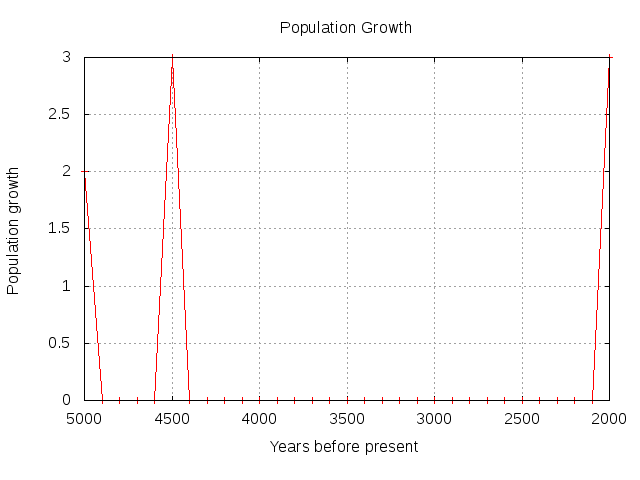
\includegraphics[width=13cm]{img/example.png}
\caption{The first example showing time periods of haplogroup
expansion.}
\end{figure}

\pagebreak


\subsection{Using the YFull Tree}

Phylogrowth is especially well suited for the use of the YFull
tree \cite{YFullTree}. It's TMRCA estimates are based on SNP
counting and calibrated by ancient and modern DNA samples
\cite{YFullMutationRate}.

As a more sophisticated example let us calculate the number of
new lineages for the P312 haplogroup. P312 is widespread in Western
Europe and most common in Spain, France and on the British Isles.

\begin{enumerate}
\item Go to the YFull R1b tree at
	\href{https://yfull.com/tree/R1b/}{https://yfull.com/tree/R1b/}.
\item Copy the tree directly from the Web page and save it
	to a text file named \emph{yfull-tree.txt}.
	Be careful that the indentations are preserved.
\item Go to a command line and type:\\
	\texttt{phylogrowth -treein=yfull-tree.txt -subclade=P312 -pngout=P312.png}
\item Done! Now watch \emph{P312.png}. Can you spot the Bronze Age
	expansion, the Roman Empire and the Migration Period?
\end{enumerate}


\begin{figure}[ht]
\centering
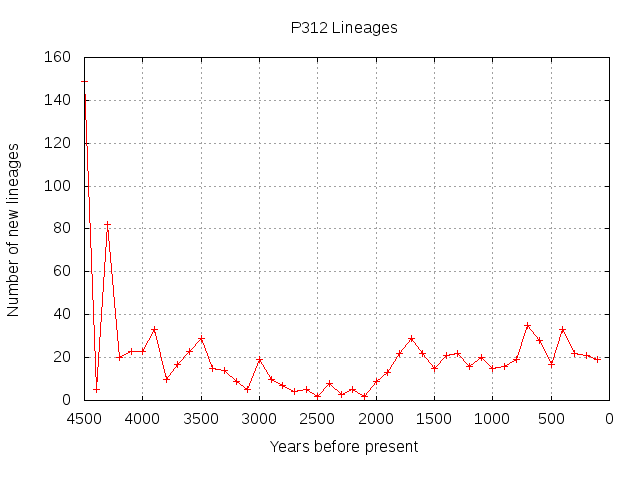
\includegraphics[width=13cm]{img/P312.png}
\caption{Number of new lineages of the P312 haplogroup.}
\end{figure}






